\documentclass{cumcmthesis} %去掉封面与编号页,电子版提交的时候使用。

%% 在这里定义标题
\title{基于{\TeX{}}的数学建模论文排版}

\begin{document}

\maketitle

\begin{abstract}

    问题背景.........................

    \textbf{针对问题一:}
    这是一个中文段落,用于测试 LaTeX 中的中文排版。希望这段文字能展示出正确的格式和样式。这里我们会继续添加一些随机的内容,以便更好地展示效果。我们可以使用许多不同的句子来填充段落,使其看起来更像真正的文本。最后,再加上一些补充说明,确保段落长度适中。

    \textbf{针对问题二:}

    \textbf{针对问题三:}

    \textbf{针对问题四:}

    
    \keywords{\textbf{关键词1} \quad \textbf{图片} \quad  \textbf{表格} \quad \textbf{公式}}

\end{abstract}

\newpage
\section{问题重述}

\subsection{问题背景}

这是一个中文段落,用于测试 LaTeX 中的中文排版。希望这段文字能展示出正确的格式和样式。这里我们会继续添加一些随机的内容,以便更好地展示效果。我们可以使用许多不同的句子来填充段落,使其看起来更像真正的文本。最后,再加上一些补充说明,确保段落长度适中。

这是一个中文段落,用于测试 LaTeX 中的中文排版。希望这段文字能展示出正确的格式和样式。这里我们会继续添加一些随机的内容,以便更好地展示效果。

\subsection{问题提出}

这是怎么回事

% 临时调整缩进的 enumerate 环境
\begin{list}{1.}{\setlength{\leftmargin}{2em}\setlength{\itemsep}{0pt}}
    \item 这是调整后的第一点
    \item 这是调整后的第二点
    \item 这是调整后的第三点
\end{list}

\begin{enumerate}[1.]\setlength{\itemsep}{0pt}
    \item 这是第一点
    \item 这是第二点
    \item 这是第三点
\end{enumerate}

\section{问题分析}

这是一个中文段落,用于测试 LaTeX 中的中文排版。希望这段文字能展示出正确的格式和样式。这里我们会继续添加一些随机的内容,以便更好地展示效果。我们可以使用许多不同的句子来填充段落,使其看起来更像真正的文本。最后,再加上一些补充说明,确保段落长度适中。

\section{模型假设}

这是一个中文段落,用于测试 LaTeX 中的中文排版。希望这段文字能展示出正确的格式和样式。这里我们会继续添加一些随机的内容,以便更好地展示效果。我们可以使用许多不同的句子来填充段落,使其看起来更像真正的文本。最后,再加上一些补充说明,确保段落长度适中。

\section{符号说明}

\setcounter{table}{-1} % 表格计数器-1

\begin{center}%htbp表示的意思是latex会尽量满足排在前面的浮动格式,就是h-t-b-p这个顺序,让排版的效果尽量好。
    \begin{longtable}{p{3.5cm}<{\centering}p{10cm}<{\centering}}
        %指定单元格宽度, 并且水平居中。
        \toprule[1.5pt]
        符号  & 说明   \\ %换行 
        \midrule
        $ a $ & 加速度 \\
        $ a $ & 加速度 \\
        $ a $ & 加速度 \\
        $ a $ & 加速度 \\
        \bottomrule[1.5pt]
    \end{longtable}
\end{center}


\section{模型的建立与求解}

\subsection{问题一模型的建立和求解}

\subsubsection{问题一模型建立}

\subsubsection{问题一结果}

\subsubsection{模型检验}

如果想强调部分内容,可以使用加粗的手段来实现。加粗字体可以用
\verb|\textbf{加粗}| 来实现。例如:\textbf{这是加粗的字体。 This is bold fonts} 。



\subsection{问题二模型的建立和求解}

\subsection{问题三模型的建立和求解}


\section{模型检验与误差分析}

这是一个中文段落,用于测试 LaTeX 中的中文排版。希望这段文字能展示出正确的格式和样式。这里我们会继续添加一些随机的内容,以便更好地展示效果。我们可以使用许多不同的句子来填充段落,使其看起来更像真正的文本。最后,再加上一些补充说明,确保段落长度适中。

\section{模型的评价、改进与推广}


\subsection{模型的优点}


中文字体没有斜体设计,但是英文字体有。\textit{斜体 Italics}。


引用样式\cite{司守奎} 引用样式\upcite{ts1} 引用样式\supercite{ts2}


%% ! 参考文献这里可以手动另起一页
\newpage 

%参考文献
\bibliographystyle{unsrt} %规定了参考文献的格式
\begin{center}
    \bibliography{reference} %调出LaTeX生成参考文献列表
\end{center}

\newpage
%附录
\begin{appendices}

    \section{支撑材料列表}

    \begin{itemize}
        \item /code:包括问题的求解源代码,均为python文件。
              \begin{itemize}
                  \item Q1.py: 对问题一的求解代码。
                  \item Q2.py: 对问题二的求解代码。
                  \item Q3.py: 对问题三的求解代码。
                  \item Q4.py: 对问题四的求解代码。
              \end{itemize}
        \item /data:包括对题目所给的数据文件进行处理后的文件,同时设置为相对路径以用来代码运行时调用。
        \item /img:包括解决问题中出现的图片文件,部分显示在论文中。
    \end{itemize}

    \section{附加代码}


    \subsubsection*{python代码}
    \lstinputlisting[
        style = Python,
        label       =   {code1}
    ]{code/1.py}

    \subsubsection*{matlab代码}
    \lstinputlisting[
        style = Matlab,
        label       =   {code2}
    ]{code/1.m}

\end{appendices}

\section{临时展示效果}

\textbf{这里是一些插图展示},插个图先

\begin{figure}[H]
    \centering
    
\includegraphics[width= 0.6\textwidth]{img/cat.pdf}
    \caption{这是一张图片}
    \label{fig1}
\end{figure}


\begin{figure}[H]
    \centering
    \begin{minipage}[c]{0.3\textwidth}
        \centering
        
\includegraphics[width=0.95\textwidth]{img/cat.pdf}
        \subcaption{流程图}
        \label{fig:sample-figure-a}
    \end{minipage}
    \begin{minipage}[c]{0.3\textwidth}
        \centering
        
\includegraphics[width=0.95\textwidth]{img/cat.pdf}
        \subcaption{流程图}
        \label{fig:sample-figure-b}
    \end{minipage}
    \begin{minipage}[c]{0.3\textwidth}
        \centering
        
\includegraphics[width=0.95\textwidth]{img/cat.pdf}
        \subcaption{流程图}
        \label{fig:sample-figure-c}
    \end{minipage}
    \caption{多图并排示例}
    \label{fig:sample-figure}
\end{figure}
这相当于整体是一张大图片,大图片引用是\cref{fig:sample-figure},子图引用别分是\cref{fig:sample-figure-a}、\cref{fig:sample-figure-b}、\cref{fig:sample-figure-c}。

% 使用cref会比ref更加快捷,cref会给出"图xx",ref只能自己写"图",再给出"xx"


\begin{figure}[H]
    \begin{minipage}[t]{0.5\textwidth}
        \centering
        
\includegraphics[width=0.9\textwidth]{img/cat.pdf}
    \end{minipage}
    \begin{minipage}[t]{0.5\textwidth}
        \centering
        
\includegraphics[width=0.9\textwidth]{img/cat.pdf}
    \end{minipage} \\ % 在这里换行相当于就是让排的图片换行了,连着写才能排四个
    \begin{minipage}[t]{0.5\textwidth}
        \centering
        
\includegraphics[width=0.9\textwidth]{img/cat.pdf}
    \end{minipage}
    \begin{minipage}[t]{0.5\textwidth}
        \centering
        
\includegraphics[width=0.9\textwidth]{img/cat.pdf}
    \end{minipage}
    \caption{演示4排图片}
\end{figure}


\begin{table}[H]
    \centering
    \setlength{\belowcaptionskip}{3pt} % 调整与标题的间距
    \renewcommand\arraystretch{1} % 调整表格行高
    \setlength{\tabcolsep}{10mm} % 设置行宽
    \caption{这是个表}
    \label{}
    \begin{tabular}{ccc}
        \toprule[1.5pt]
        这是三线表 & nb         & ???        \\
        \midrule
        这是一个   & 这是另一个 & 使用三线表 \\
        \bottomrule[1.5pt]
    \end{tabular}
\end{table}

\begin{tcode}
    \begin{table}[H]
        \caption[标签名]{中文标题}
        \begin{tabular}{cc...c}
            \toprule[1.5pt]
            表头第1个格   & 表头第2个格   & ... & 表头第n个格   \\
            \midrule[1pt]
            表中数据(1,1) & 表中数据(1,2) & ... & 表中数据(1,n) \\
            表中数据(2,1) & 表中数据(2,2) & ... & 表中数据(2,n) \\
            ................................................... \\
            表中数据(m,1) & 表中数据(m,2) & ... & 表中数据(m,n) \\
            \bottomrule[1.5pt]
        \end{tabular}
    \end{table}
\end{tcode}



\begin{enumerate}[1.]\setlength{\itemsep}{0pt}
    \item 1
    \item    f
    \item
\end{enumerate}

% Please add the following required packages to your document preamble:
% \usepackage{graphicx}
\begin{table}[H]
    \centering
    \caption{\href{https://www.tablesgenerator.com/latex_tables}{网站生成图表,点击进入}}
    \label{tab:my-table}
    \resizebox{\textwidth}{!}{%
        \begin{tabular}{|l|l|l|l|}
            \hline
            标准角度与实际的差 & 倾斜角度 & 标准角度与实际的差 & 倾斜角度 \\ \hline
                               &          &                    &          \\ \hline
                               &          &                    &          \\ \hline
                               &          &                    &          \\ \hline
                               &          &                    &          \\ \hline
                               &          &                    &          \\ \hline
        \end{tabular}%
    }
\end{table}


\textbf{使用矩阵排版}
\[
    \begin{matrix}
        1         & 0.3420047 & 0.3339529 & 0.3381766 & 0.3362277 & 0.3547872   & 0.3355143 \\
        0.3374153 & 0.4495615 & 0.3652695 & 0.3334384 & 0.334335  & 0.333648433 & 0.3340383 \\
    \end{matrix}
\]

\textbf{下面是多排表格}

\begin{table}[H]
    \caption{这是多排表格的标题}
    \begin{minipage}[t]{0.48\textwidth}
        \centering
        \setlength{\belowcaptionskip}{3pt} % 调整与标题的间距
        \renewcommand\arraystretch{1} % 调整表格行高
        \setlength{\tabcolsep}{4mm} % 设置行宽
        \label{}
        \begin{tabular}{ccc}
            \toprule[1.5pt]
                     & 这是表格  & 非常不错 \\
            \midrule
            good     & 1.000 & 0.080    \\
            nice & 0.080 & 1.000    \\
            \bottomrule[1.5pt]
        \end{tabular}
    \end{minipage} % 在这里换行相当于就是让排的图片换行了,连着写才能排四个
    \begin{minipage}[t]{0.48\textwidth}
        \centering
        \setlength{\belowcaptionskip}{3pt} % 调整与标题的间距
        \renewcommand\arraystretch{1} % 调整表格行高
        \setlength{\tabcolsep}{4mm} % 设置行宽
        \label{}
        \begin{tabular}{ccc}
            \toprule[1.5pt]
                     & 这是表格  & 非常不错 \\
            \midrule
            good     & 1.000 & 0.080    \\
            nice & 0.080 & 1.000    \\
            \bottomrule[1.5pt]
        \end{tabular}
    \end{minipage}
\end{table}

\begin{figure}[H]
    \centering
    \makebox[\textwidth][c]{
\includegraphics[width= 1.3\textwidth]{img/cat.pdf}}
    \caption{这是测试,这里可以插入较大图片}
\end{figure}

\begin{figure}[H]
    \centering
    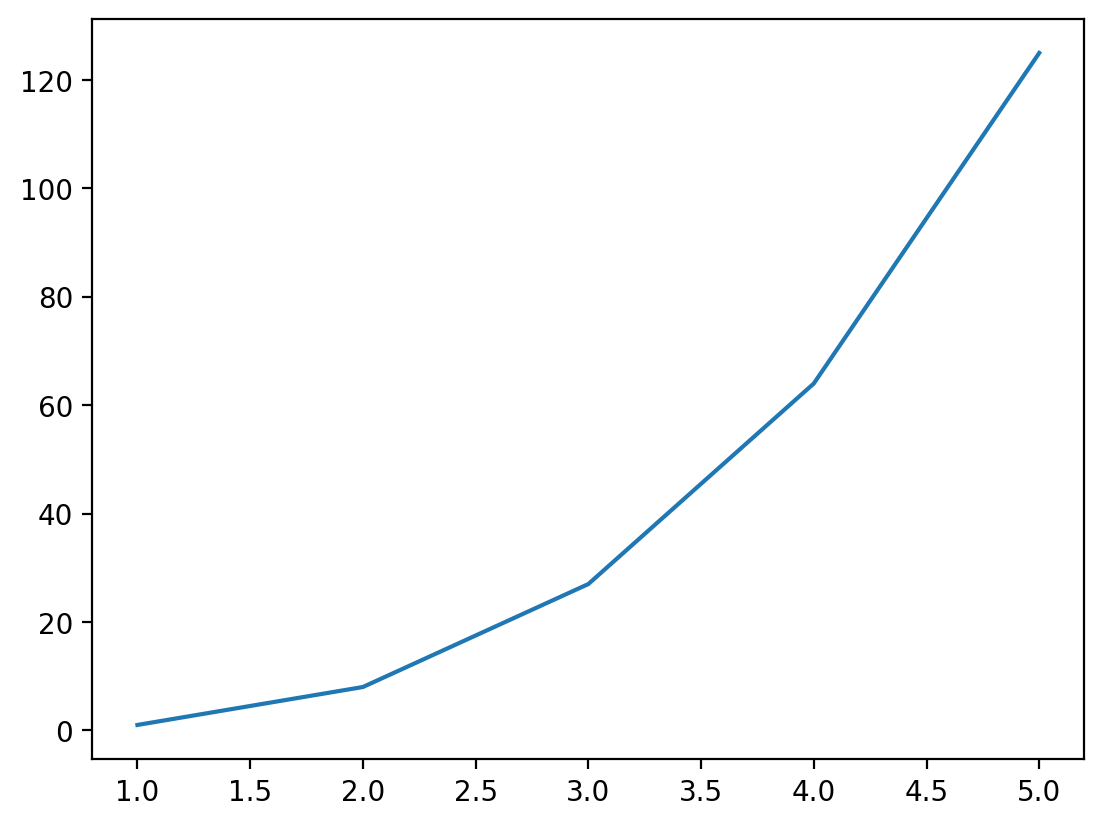
\includegraphics[width= 1\textwidth]{img/1.png}
    \caption{插入图片}
\end{figure}

\end{document}